\documentclass[journal,12pt,twocolumn]{IEEEtran}
%
\usepackage{setspace}
\usepackage{gensymb}
\usepackage{siunitx}
\usepackage{tkz-euclide} 
\usepackage{textcomp}
\usepackage{standalone}
\usetikzlibrary{calc}
\newcommand\hmmax{0}
\newcommand\bmmax{0}

%\doublespacing
\singlespacing

%\usepackage{graphicx}
%\usepackage{amssymb}
%\usepackage{relsize}
\usepackage[cmex10]{amsmath}
%\usepackage{amsthm}
%\interdisplaylinepenalty=2500
%\savesymbol{iint}
%\usepackage{txfonts}
%\restoresymbol{TXF}{iint}
%\usepackage{wasysym}
\usepackage{amsthm}
%\usepackage{iithtlc}
\usepackage{mathrsfs}
\usepackage{txfonts}
\usepackage{stfloats}
\usepackage{bm}
\usepackage{cite}
\usepackage{cases}
\usepackage{subfig}
%\usepackage{xtab}
\usepackage{longtable}
\usepackage{multirow}
%\usepackage{algorithm}
%\usepackage{algpseudocode}
\usepackage{enumitem}
\usepackage{mathtools}
\usepackage{steinmetz}
\usepackage{tikz}
\usepackage{circuitikz}
\usepackage{verbatim}
\usepackage{tfrupee}
\usepackage[breaklinks=true]{hyperref}
%\usepackage{stmaryrd}
\usepackage{tkz-euclide} % loads  TikZ and tkz-base
%\usetkzobj{all}
\usetikzlibrary{calc,math}
\usepackage{listings}
    \usepackage{color}                                            %%
    \usepackage{array}                                            %%
    \usepackage{longtable}                                        %%
    \usepackage{calc}                                             %%
    \usepackage{multirow}                                         %%
    \usepackage{hhline}                                           %%
    \usepackage{ifthen}                                           %%
  %optionally (for landscape tables embedded in another document): %%
    \usepackage{lscape}     
\usepackage{multicol}
\usepackage{chngcntr}
\usepackage{amsmath}
\usepackage{cleveref}
%\usepackage{enumerate}

%\usepackage{wasysym}
%\newcounter{MYtempeqncnt}
\DeclareMathOperator*{\Res}{Res}
%\renewcommand{\baselinestretch}{2}
\renewcommand\thesection{\arabic{section}}
\renewcommand\thesubsection{\thesection.\arabic{subsection}}
\renewcommand\thesubsubsection{\thesubsection.\arabic{subsubsection}}

\renewcommand\thesectiondis{\arabic{section}}
\renewcommand\thesubsectiondis{\thesectiondis.\arabic{subsection}}
\renewcommand\thesubsubsectiondis{\thesubsectiondis.\arabic{subsubsection}}

% correct bad hyphenation here
\hyphenation{op-tical net-works semi-conduc-tor}
\def\inputGnumericTable{}                                 %%

\lstset{
%language=C,
frame=single, 
breaklines=true,
columns=fullflexible
}
%\lstset{
%language=tex,
%frame=single, 
%breaklines=true
%}
\usepackage{graphicx}
\usepackage{pgfplots}

\begin{document}


\newtheorem{theorem}{Theorem}[section]
\newtheorem{problem}{Problem}
\newtheorem{proposition}{Proposition}[section]
\newtheorem{lemma}{Lemma}[section]
\newtheorem{corollary}[theorem]{Corollary}
\newtheorem{example}{Example}[section]
\newtheorem{definition}[problem]{Definition}
%\newtheorem{thm}{Theorem}[section] 
%\newtheorem{defn}[thm]{Definition}
%\newtheorem{algorithm}{Algorithm}[section]
%\newtheorem{cor}{Corollary}
\newcommand{\BEQA}{\begin{eqnarray}}
\newcommand{\EEQA}{\end{eqnarray}}
\newcommand{\define}{\stackrel{\triangle}{=}}
\bibliographystyle{IEEEtran}
%\bibliographystyle{ieeetr}
\providecommand{\mbf}{\mathbf}
\providecommand{\abs}[1]{\ensuremath{\left\vert#1\right\vert}}
\providecommand{\norm}[1]{\ensuremath{\left\lVert#1\right\rVert}}
\providecommand{\mean}[1]{\ensuremath{E\left[ #1 \right]}}
\providecommand{\pr}[1]{\ensuremath{\Pr\left(#1\right)}}
\providecommand{\qfunc}[1]{\ensuremath{Q\left(#1\right)}}
\providecommand{\sbrak}[1]{\ensuremath{{}\left[#1\right]}}
\providecommand{\lsbrak}[1]{\ensuremath{{}\left[#1\right.}}
\providecommand{\rsbrak}[1]{\ensuremath{{}\left.#1\right]}}
\providecommand{\brak}[1]{\ensuremath{\left(#1\right)}}
\providecommand{\lbrak}[1]{\ensuremath{\left(#1\right.}}
\providecommand{\rbrak}[1]{\ensuremath{\left.#1\right)}}
\providecommand{\cbrak}[1]{\ensuremath{\left\{#1\right\}}}
\providecommand{\lcbrak}[1]{\ensuremath{\left\{#1\right.}}
\providecommand{\rcbrak}[1]{\ensuremath{\left.#1\right\}}}
\theoremstyle{remark}
\newtheorem{rem}{Remark}
\newcommand{\sgn}{\mathop{\mathrm{sgn}}}
\providecommand{\res}[1]{\Res\displaylimits_{#1}} 
%\providecommand{\norm}[1]{\lVert#1\rVert}
\providecommand{\mtx}[1]{\mathbf{#1}}
\providecommand{\fourier}{\overset{\mathcal{F}}{ \rightleftharpoons}}
%\providecommand{\hilbert}{\overset{\mathcal{H}}{ \rightleftharpoons}}
\providecommand{\system}{\overset{\mathcal{H}}{ \longleftrightarrow}}
	%\newcommand{\solution}[2]{\textbf{Solution:}{#1}}
\newcommand{\solution}{\noindent \textbf{Solution: }}
\newcommand{\cosec}{\,\text{cosec}\,}
\providecommand{\dec}[2]{\ensuremath{\overset{#1}{\underset{#2}{\gtrless}}}}
\newcommand{\myvec}[1]{\ensuremath{\begin{pmatrix}#1\end{pmatrix}}}
\newcommand{\mydet}[1]{\ensuremath{\begin{vmatrix}#1\end{vmatrix}}}
%\numberwithin{equation}{section}
\numberwithin{equation}{subsection}
%\numberwithin{problem}{section}
%\numberwithin{definition}{section}
\makeatletter
\@addtoreset{figure}{problem}
\makeatother
\let\StandardTheFigure\thefigure
\let\vec\mathbf
%\renewcommand{\thefigure}{\theproblem.\arabic{figure}}
\renewcommand{\thefigure}{\theproblem}
%\setlist[enumerate,1]{before=\renewcommand\theequation{\theenumi.\arabic{equation}}
%\counterwithin{equation}{enumi}
%\renewcommand{\theequation}{\arabic{subsection}.\arabic{equation}}
\def\putbox#1#2#3{\makebox[0in][l]{\makebox[#1][l]{}\raisebox{\baselineskip}[0in][0in]{\raisebox{#2}[0in][0in]{#3}}}}
     \def\rightbox#1{\makebox[0in][r]{#1}}
     \def\centbox#1{\makebox[0in]{#1}}
     \def\topbox#1{\raisebox{-\baselineskip}[0in][0in]{#1}}
     
 \vspace{3cm}
 \title{Assignment 4}
 \author{Matish Singh Tanwar}
 \maketitle
 \newpage
 \bigskip
 %\renewcommand{\thefigure}{\theenumi}
 \renewcommand{\thetable}{\theenumi}
\vspace{1.0cm}
\begin{abstract}
This document solves question based on triangle.
\end{abstract}
\vspace{0.5cm}
%
Download all latex-tikz codes from 
\begin{lstlisting}
https://github.com/Matish007/Matrix-Theory-EE5609-/tree/master/Assignment_4
\end{lstlisting}
%
\vspace{0.5mm}
\section{Problem}
Line L is the bisector of $\angle{A}$ and B is any point on L.BP and BQ are perpendiculars from B to the arms of $\angle{A}$.Show that:-
\begin{align}
    a) &\quad \triangle APB \cong\triangle AQB\\
    b) & \quad BP=BQ
\end{align}
\renewcommand{\thefigure}{1}
\begin{figure}[!ht]
\centering
\resizebox{\columnwidth}{!}{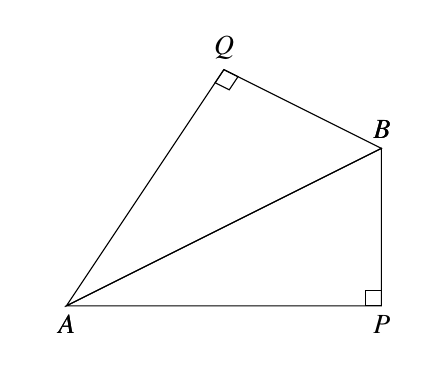
\begin{tikzpicture} 
        \coordinate (P) at (4, 0) {};
        \coordinate (A) at (0, 0) {};
        \coordinate (B) at (4, 2) {};
        \coordinate (Q) at (2, 3) {};
        \draw (Q)node[above]{$Q$}--(A)node[below]{$A$}--(B)node[above]{$B$}--cycle;
        \draw (B)node[above]{$B$}--(A)node[below]{$A$}--(P)node[below]{$P$}--cycle;
\tkzMarkRightAngle[size=.2](B,P,A);
\tkzLabelAngle[dist=.5](P,A,B){};
\tkzMarkRightAngle[size=.2](B,Q,A);
\tkzLabelAngle[dist=.5](Q,A,B){};
\end{tikzpicture}
}
\caption{figure}
\label{fig1}
\end{figure}
\section{Explanation}
Given:-
\begin{align}
  \angle{BAP}=\angle{BAQ}=\alpha\label{1}\\ 
    \angle{AQB}=\angle{APB}\label{2}
\end{align}
In $\triangle ABQ$
\begin{align}
    \angle{ABQ} + \angle{AQB} + \angle{BAQ}=180\degree\label{3}
\end{align}
In $\triangle ABP$
\begin{align}
    \angle{ABP} + \angle{APB} + \angle{BAP}=180\degree\label{4}
\end{align}
Subtracting \eqref{3} and \eqref{4} and using \eqref{1} and \eqref{2} we get,
\begin{align}
\angle{ABQ}=\angle{ABP}
\end{align}
Since,line BP and BQ are perpendicular to AP and AQ respectively..So,their respective dot product will be zero.We get,
\begin{align}
    (\vec{B}-\vec{Q})^T(\vec{A}-\vec{Q})=0\label{5}\\
    (\vec{B}-\vec{P})^T(\vec{A}-\vec{P})=0\label{6}
\end{align}
We know that,$(\vec{B}-\vec{P})^T(\vec{B}-\vec{P})$ = $\norm{\vec{B}-\vec{P}}^2$\\
 Also let
 \begin{align}
 \norm{\vec{B}-\vec{A}}^2 = k^2\label{7}
 \end{align}
\begin{align}
(\vec{B}-\vec{P})^T(\vec{B}-\vec{P})=(\vec{B}-\vec{A}+\vec{A}-\vec{P})^T(\vec{B}-\vec{A}+\vec{A}-\vec{P})
\end{align}
\begin{align}
 \begin{split}
\norm{\vec{B}-\vec{P}}^2=(\vec{B}-\vec{A})^T(\vec{B}-\vec{A})\\
+(\vec{A}-\vec{P})^T(\vec{A}-\vec{P})\\
+(\vec{A}-\vec{P})^T(\vec{B}-\vec{A})\\
+(\vec{B}-\vec{A})^T(\vec{A}-\vec{P})\\
=\norm{\vec{B}-\vec{A}}^2 + \norm{\vec{A}-\vec{P}}^2\\ 
  + 2\norm{\vec{A}-\vec{P}}\norm{\vec{B}-\vec{A}}\cos\alpha\label{8}
  \end{split}
\end{align}
\begin{align}
\begin{split}
 (\vec{A}-\vec{P})^T(\vec{B}-\vec{A})=(\vec{B}-\vec{A})^T(\vec{A}-\vec{P})\\
 = \norm{\vec{A}-\vec{P}} \norm{\vec{B}-\vec{A}} \cos\alpha\label{18}
\end{split}
\end{align}
Substituting \eqref{18}, \eqref{7} in \eqref{8} we get,
\begin{align}
  \begin{split}
      \norm{\vec{B}-\vec{P}}^2=k^2+\norm{\vec{A}-\vec{P}}^2
      +2k\norm{\vec{A}-\vec{P}}\cos\alpha\label{14}
  \end{split}  
\end{align}
Similarly,we get
\begin{align}
    \norm{\vec{B}-\vec{Q}}^2=k^2+\norm{\vec{A}-\vec{Q}}^2
      +2k\norm{\vec{A}-\vec{Q}}\cos\alpha\label{15}
\end{align}
\begin{align}
    \cos\alpha = \frac{(\vec{B}-\vec{A})^T(\vec{P}-\vec{A})}{k\norm{\vec{P}-\vec{A}}} = \frac{(\vec{B}-\vec{A})^T(\vec{Q}-\vec{A})}{k\norm{\vec{Q}-\vec{A}}}\label{13}\\
    (\vec{B}-\vec{A})^T(\vec{P}-\vec{A})=(\vec{B}-\vec{P}+\vec{P}-\vec{A})^T(\vec{P}-\vec{A})\\
    \implies (\vec{B}-\vec{P})^T(\vec{P}-\vec{A}) + \norm{\vec{P}-\vec{A}}^2\label{9}\\
    (\vec{B}-\vec{A})^T(\vec{Q}-\vec{A})=(\vec{B}-\vec{Q}+\vec{Q}-\vec{A})^T(\vec{Q}-\vec{A})\\
     \implies (\vec{B}-\vec{Q})^T(\vec{Q}-\vec{A}) + \norm{\vec{Q}-\vec{A}}^2\label{10}
\end{align}
Substituting \eqref{5} and \eqref{6} in \eqref{10} and \eqref{9} respectively we get,
\begin{align}
    (\vec{B}-\vec{A})^T(\vec{P}-\vec{A})=\norm{\vec{P}-\vec{A}}^2\label{11}\\
    (\vec{B}-\vec{A})^T(\vec{Q}-\vec{A})=\norm{\vec{Q}-\vec{A}}^2\label{12}
\end{align}
Substituting \eqref{11} and \eqref{12} in \eqref{13} we get,
\begin{align}
    \cos\alpha=\norm{\vec{P}-\vec{A}}=\norm{\vec{Q}-\vec{A}}\label{16}
\end{align}
Substituting \eqref{16} in \eqref{14} and \eqref{15} we get,
\begin{align}
    \norm{\vec{B}-\vec{P}}=\norm{\vec{B}-\vec{Q}}\label{17}
\end{align}
From \eqref{17} we can say that $\vec{B}$ is equidistant from the arms of $\angle{A}$,where $\vec{P}$ and $\vec{Q}$ are the points on the arms of $\angle{A}$
Using \eqref{1},\eqref{2},\eqref{17} and by AAS(Angle Angle Side) property of congruency we can say that:-\\
\begin{align}
\triangle APB \cong \triangle AQB
\end{align}
\end{document}
